% paper/sections/12d_highre_dccd.tex
%
% §12.3c  高 Re 安定性：DCCD フィルタの非侵襲性
% ═══════════════════════════════════════════════════════════════════════════════
\subsubsection{高 Re 安定性：DCCD フィルタの非侵襲性}
\label{sec:highre_dccd}
% ═══════════════════════════════════════════════════════════════════════════════

\noindent\textbf{動機：}
§~\ref{sec:ns_time_accuracy} の精度検証は等密度・周期境界の理想条件で実施した．
次節（§~\ref{sec:advection_pressure_coupling}）の二相流テストでは境界層・界面・高密度比を含む
複雑条件で DCCD を使用するため，フィルタが実流体流動の物理精度を損なわないことを
事前に確認する必要がある．

\noindent\textbf{目的：}
DCCD の 10 次選択的散逸（§~\ref{sec:dccd_filter_theory}）が，
高 Reynolds 数流れにおいて物理的精度を損なわないことを NS パイプライン全体で確認する．

\noindent\textbf{評価対象：}
CCD（$\varepsilon_d = 0$，フィルタなし）と
DCCD（$\varepsilon_d = 0.05$，10 次フィルタ）の
運動エネルギー保存性・安定性の比較．

\noindent\textbf{手順とパラメタ：}
\begin{itemize}[noitemsep]
  \item 二重剪断層（Double shear layer）：
        $u = \tanh\bigl((y - \pi/2)/\delta\bigr)$（$y \leq \pi$），
        $u = \tanh\bigl((3\pi/2 - y)/\delta\bigr)$（$y > \pi$），
        $v = \varepsilon_0\sin x$，$\delta = \pi/15$，$\varepsilon_0 = 0.05$
  \item 計算領域 $[0, 2\pi]^2$，周期境界条件
  \item $\mathit{Re} = 1000$（$\nu = 10^{-3}$），$T = 0.5$
  \item 格子 $N = 64, 128$，AB2+IPC，FFT 直接法 PPE（周期境界の等密度 Poisson を FFT で厳密求解）\footnote{$N = 256$ は CFL 制約により計算コストが大きく，$N = 64, 128$ で非侵襲性の収束傾向を十分確認できたため省略した．}
\end{itemize}

\noindent\textbf{結果：}

\begin{table}[htbp]
\centering
\caption{高 Re 二重剪断層テスト：CCD vs DCCD（$\mathit{Re} = 1000$）}
\label{tab:highre_dccd}
\renewcommand{\arraystretch}{1.3}
\begin{tabular}{rlrcl}
\toprule
$N$ & スキーム & $E_k(T)$ & $|E_k^{\text{CCD}} - E_k^{\text{DCCD}}| / E_k^{\text{CCD}}$ & 判定 \\
\midrule
  64 & CCD\, ($\varepsilon_d{=}0$)    & $1.709236 \times 10^{1}$ & \multirow{2}{*}{$1.5 \times 10^{-8}$} & 安定 \\
  64 & DCCD ($\varepsilon_d{=}0.05$) & $1.709236 \times 10^{1}$ &  & 安定 \\
\midrule
 128 & CCD\, ($\varepsilon_d{=}0$)    & $1.709233 \times 10^{1}$ & \multirow{2}{*}{$8.7 \times 10^{-9}$} & 安定 \\
 128 & DCCD ($\varepsilon_d{=}0.05$) & $1.709233 \times 10^{1}$ &  & 安定 \\
\bottomrule
\end{tabular}
\end{table}

\noindent\textbf{結論：}
$N = 64, 128$ の両格子で CCD と DCCD の $E_k(T)$ 相対差は $10^{-8}$--$10^{-9}$ であり，
DCCD の 10 次選択的散逸が低波数の物理モード（渦構造）を保存していることを確認した
（§~\ref{sec:dccd_filter_theory} の分散関係解析と整合）．
DCCD フィルタが物理的精度を損なわずに Nyquist モード近傍の高周波雑音のみを選択的に減衰する
\textbf{非侵襲性}が，NS パイプライン全体で成立する．

\begin{figure}[htbp]
\centering
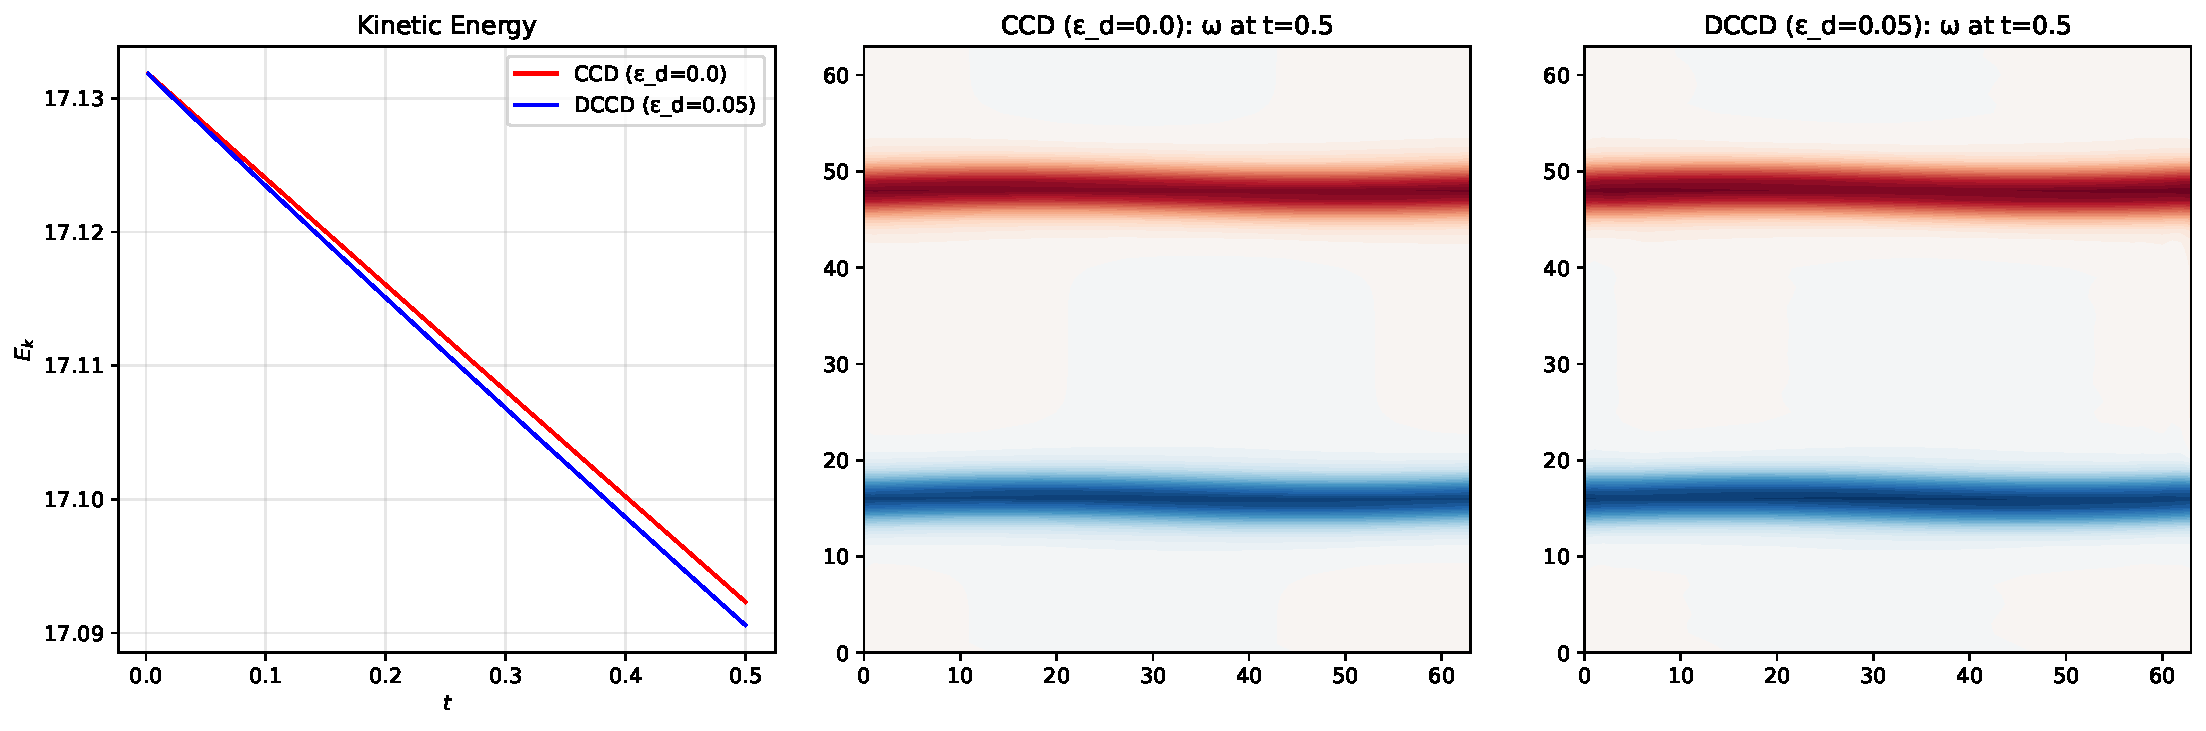
\includegraphics[width=0.88\linewidth]{figures/ch11_highre_dccd_comparison}
\caption{高 Re 二重剪断層（$\mathit{Re}=1000$）における CCD vs DCCD の渦度場・運動エネルギー比較
  （$N=64, 128$，$T=0.5$）．
  両スキームの渦構造は視覚的に一致し，$E_k$ の相対差は $\Ord{10^{-8}}$ である．}
\label{fig:highre_dccd_comparison}
\end{figure}

\noindent
以上により，§~\ref{sec:advection_pressure_coupling} 以降の二相流テストでは
DCCD を標準スキームとして使用する．
